\documentclass[10pt, conference, compsocconf]{IEEEtran}

\usepackage{color}
\usepackage{soul}

%\documentclass[a4paper, UKenglish]{lipics}
%\usepackage{amsmath}
%\theoremstyle{plain}

\usepackage{subfigure}
%\usepackage{hyperref}
\usepackage{graphicx}
\usepackage{amssymb}
\usepackage{amsmath}
\usepackage{times}
\let\proof\relax % undefine the environment
\let\endproof\relax
\usepackage{amsthm}

\usepackage{xspace}
\usepackage{algorithm}% http://ctan.org/pkg/algorithm
\usepackage[noend]{algpseudocode}% http://ctan.org/pkg/algorithmicx

\newcommand{\todo}[1]{\color{red}\textbf{\hl{\{ #1 \}}}\color{black}\xspace}
\newcommand{\ceil}[1]{\left\lceil #1 \right\rceil}
\newcommand{\floor}[1]{\left\lfloor #1 \right\rfloor}

\begin{document}
\title{Work Inefficient Partitioning: The space time kernel density case.}


\author{\IEEEauthorblockN{Erik  Saule}
\IEEEauthorblockA{ Dept. of Computer Science\\
UNC Charlotte\\
Charlotte, NC, USA\\
Email: esaule@uncc.edu}
}

\maketitle


\begin{abstract}
  In spatial problems it is common to partition the work to distribute
  it on multiple nodes or on multiple cores. The work is usually
  generated by the space itself and by points (particles in physics
  simulation) that are located in that space. Most partitioning
  techniques are assuming that the partitioning is work efficient,
  that is to say that after decomposition the total amount of work has
  not changed. We are investigating in this paper what to do when that
  assumption does not hold.

  Space-Time Kernel Density Estimation is a problem that does not
  support work efficient partitioning. We use that problem has a
  applications to motivate our work, but we believe that our
  conclusions generalize to other problem that do not support work
  efficient partitioning.

  We first show that naive over-decomposition techniques do not lead
  to desirable solutions because they do not account for the work
  inefficient partitioning. We propose optimal k-way partitioning
  based on dynamic programming and show that there may not be good
  balanced k-way partitions. To solve this problem we introduced an
  overhead-aware over-decomposition technique and explore the
  trade-off between load balance and overhead in partitioning.
\end{abstract}

\begin{IEEEkeywords}
\end{IEEEkeywords}


\IEEEpeerreviewmaketitle

\section{Introduction}

When computation is located in a spatial domain, a common technique to
make these computation parallel is to decompose the spatial domain
into subdomains so that the computation of each subdomain can be done
in parallel. Applications following that model appear in all realms of
applications of parallel computing, including physics with n-body
computation, mecanical simulations, chemistry, geography, and many others.

Algorithms for decomposing spatial located computation have attracted
a constant number of attention over the years. Some methods are
designed to be fast heuristics~\cite{RB}, while some other attempt to
at finding optimal decompositions~\cite{erdeniz}. Some deal with
heterogeneous processors~\cite{pinar}. Also fast and generic
implementation of these types of decomposition for distributed memory
machines have been provided~\cite{deveci_ipdps}.

Yet, all methods usually assume that the decomposition is work
efficient. It is not uncommon that these methods overdecompose the
spatial domain; that is to say they decompose the space in many more
domains than there are processors on the system, and rely on giving
multiple domains to each processor to achieve load balance.

Some application do not admit work efficient spatial
decomposition. That is to say, when a domain $D$ is decomposed in two
subdomains $D_1$ and $D_2$, it is possible that the sum of the work to
process $D_1$ and $D_2$ is larger than the work necessary to process
domain $D$.

As a representative of this class of application, we present here
a common geography problem. Visualizing the distibution of some events
requires to compute a Space Time Kernel Density
Estimation(STKDE)~\cite{delmelle}. Decomposing the spatial domain
(space-time domain in STKDE terminology) to process each subdomain
independently is not a work-efficient decomposition~\cite{icpp17}. As
such traditional overdecomposition techniques lead to an increase in
work which limits the usefulness of parallelism.

We present in this paper spatial decomposition techniques suitable for
problem which do not have work-efficient decomposition. By modeling
the amount of work in the different parts of a decomposition, one can
seek to find the decomposition with minimal maximum work. Because
finding an optimal decomposition for arbitrary decomposition patterns
is usually NP-hard, we focus on classes of decomposition that can be
optimized optimally in polynomial time by dynamic programing for a
given number of parts, namely jagged decomposition and recursive
decompositions in blocks.

However these decompositions only allocate a single block per
processor, which may lead to an imbalanced decomposition. We propose
an algorithm aware of work inefficience which overdecomposes the
domain for better load balance. The algorithm works by exploring a
bi-objective tradeoff between the most loaded part and the total
amount of overhead induced by the decomposition.

The remaining of the document is organized has follows.
Section~\ref{sec:relworks} presents common strategies for spatial
decomposition. Section \ref{sec:stkde} describes the Space-Time Kernel
Density Estimation problem and explain why it is
work-inefficient. Methods for decomposing the work for execution on
$P$ processors are presented in Section~\ref{sec:exactdecomposition};
while work-inefficiency aware methods are presented in
Section~\ref{sec:overdecomposition}. Practical results obtained on
real instances of STKDE are shown in
Section~\ref{sec:experiments}. Final remarks and future works are
discussed in Section~\ref{sec:ccl}.

\section{Related Works}
\label{sec:relworks}

Mostly on work efficient partition.

\section{Space time Kernel Density Estimation}
\label{sec:stkde}

\subsection{Description}

Space-time kernel density (STKDE) is used for identifying
spatiotemporal patterns in datasets. It is a temporal
extension of the traditional 2D kernel density
estimation~\cite{Silverman86} which generates density surface
(``heatmap'') from a set of $n$ points located in a geographic space. The resulting density
estimates are visualized within the space-time cube framework using two spatial $(x,
y)$ and a temporal dimension $(t)$~\cite{Nakaya10}. STKDE creates a discretized 3D
 volume where each voxel (3D equivalent of a pixel) is assigned a
density estimate based on the surrounding points. The space-time
density is estimated using (following the notations
of~\cite{Hohl16}):

$$ \hat{f} (x, y, t) = \frac{1}{n h_s^2 h_t} \sum_{i | d_i < h_s, t_i<h_t}
k_s (\frac{x-x_i}{h_s},\frac{y-y_i}{h_s}) k_t(\frac{t-t_i}{h_t})$$

Density $\hat{f} (x, y, t)$ of each voxel is determined by number and distance of events (points)
$(x_i, y_i, t_i)$ within its vicinity, which is conceptualized by a
cylinder. The spatial bandwidth $h_s$ forms a circle which, due to the
orthogonal relationship between space and time, is extended to a
cylinder by temporal bandwidth $h_t$. For every event inside the
cylinder, the spatial ($d_i$) and temporal ($t_i$) distances are smaller
than $h_s$ and $h_t$. Therefore, the event receives a weight based on the
kernel functions $k_s$ and $k_t$ (distance decay):

$$k_s (u,v) = \frac{\pi}{2} (1-u)^2 (1-v)^2$$
$$k_t (w) = \frac{3}{4} (1-w)^2$$

Figure~\ref{fig:stkde-ex} illustrates how varying the bandwidths used
in STKDE helps focusing the graphical visualization of Dengue fever
cases in Cali, Colombia~\cite{Delmelle14}. Figure~\ref{fig:stkde} shows the impact
of a single point on the neighboring space.

\begin{figure}
%  \subfigure[$h_s = 2500m$, $h_t = 14 days$]{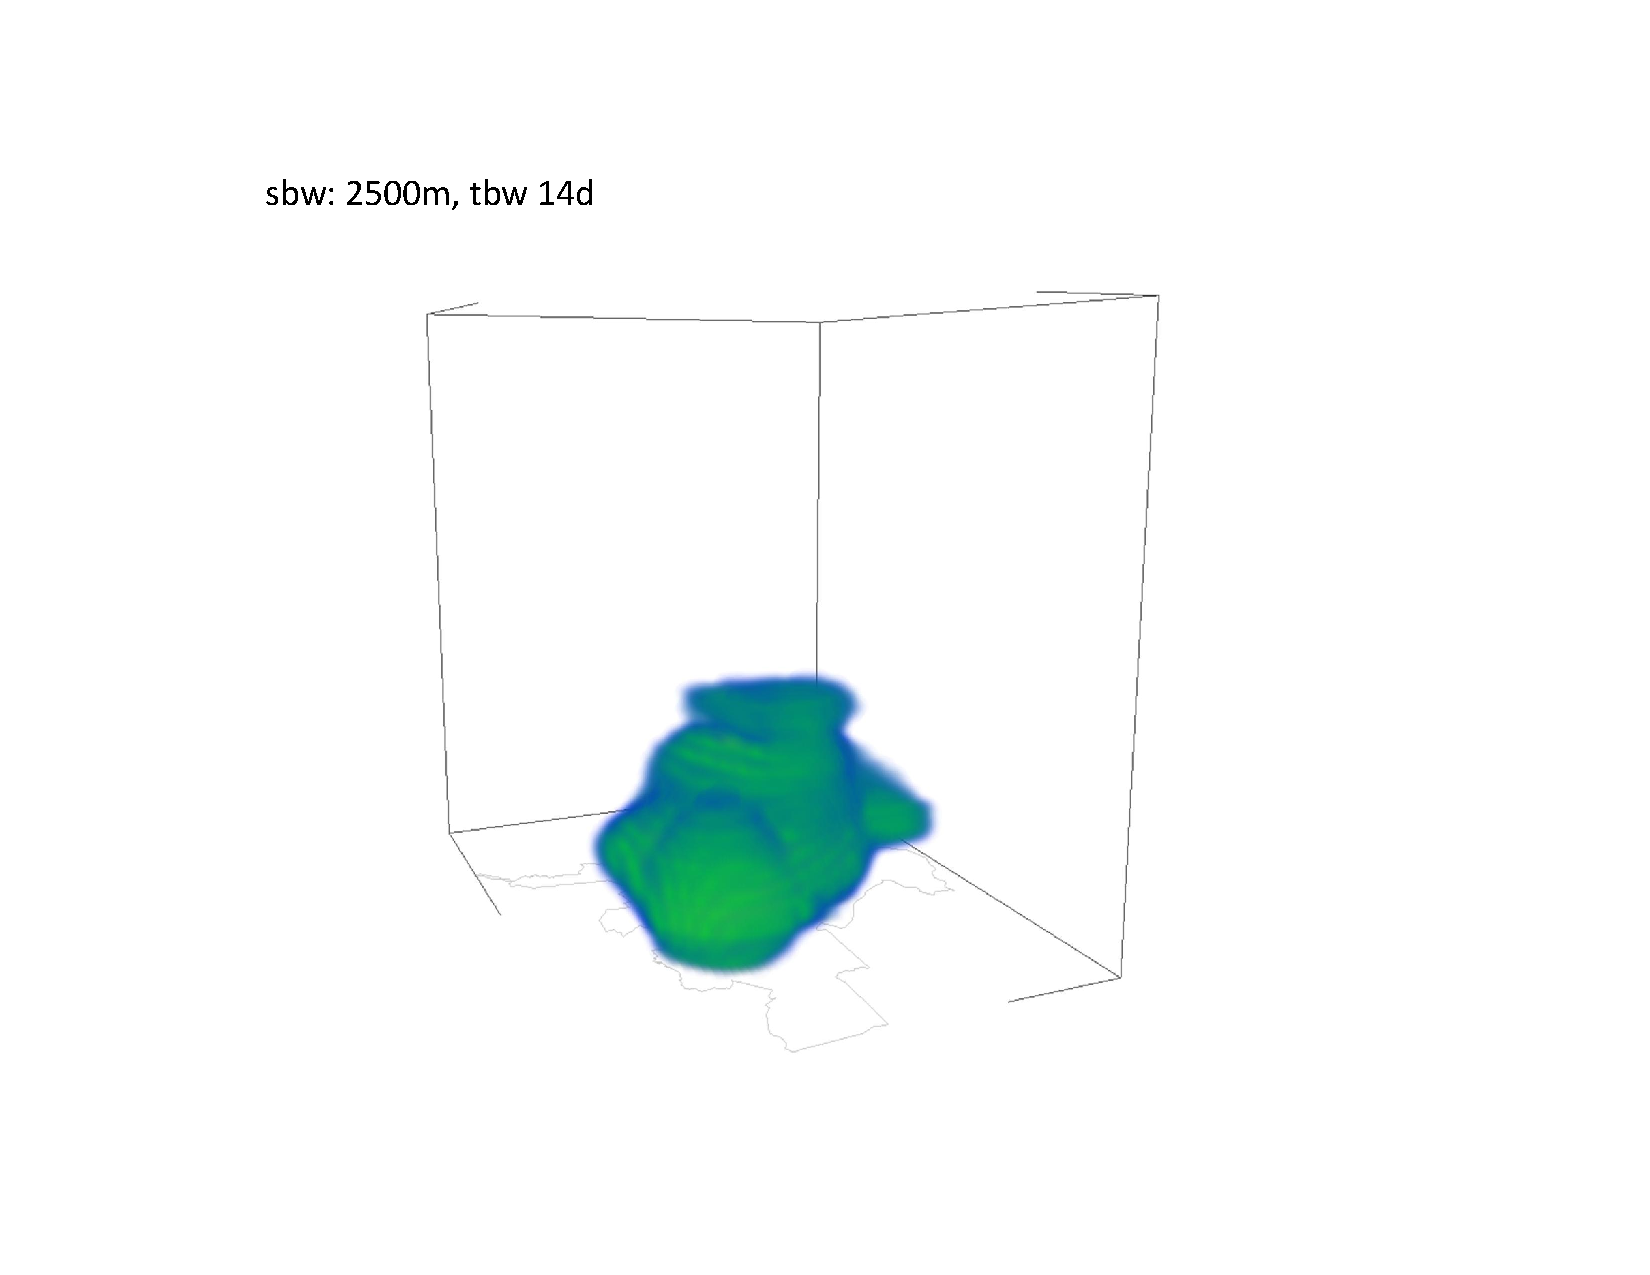
\includegraphics[page=1, width=.45\linewidth, trim={8cm 3.8cm 8cm 10cm}, clip]{figures/dengue-viz.pdf}}
  \subfigure[$h_s = 2500m$, $h_t = 14 days$]{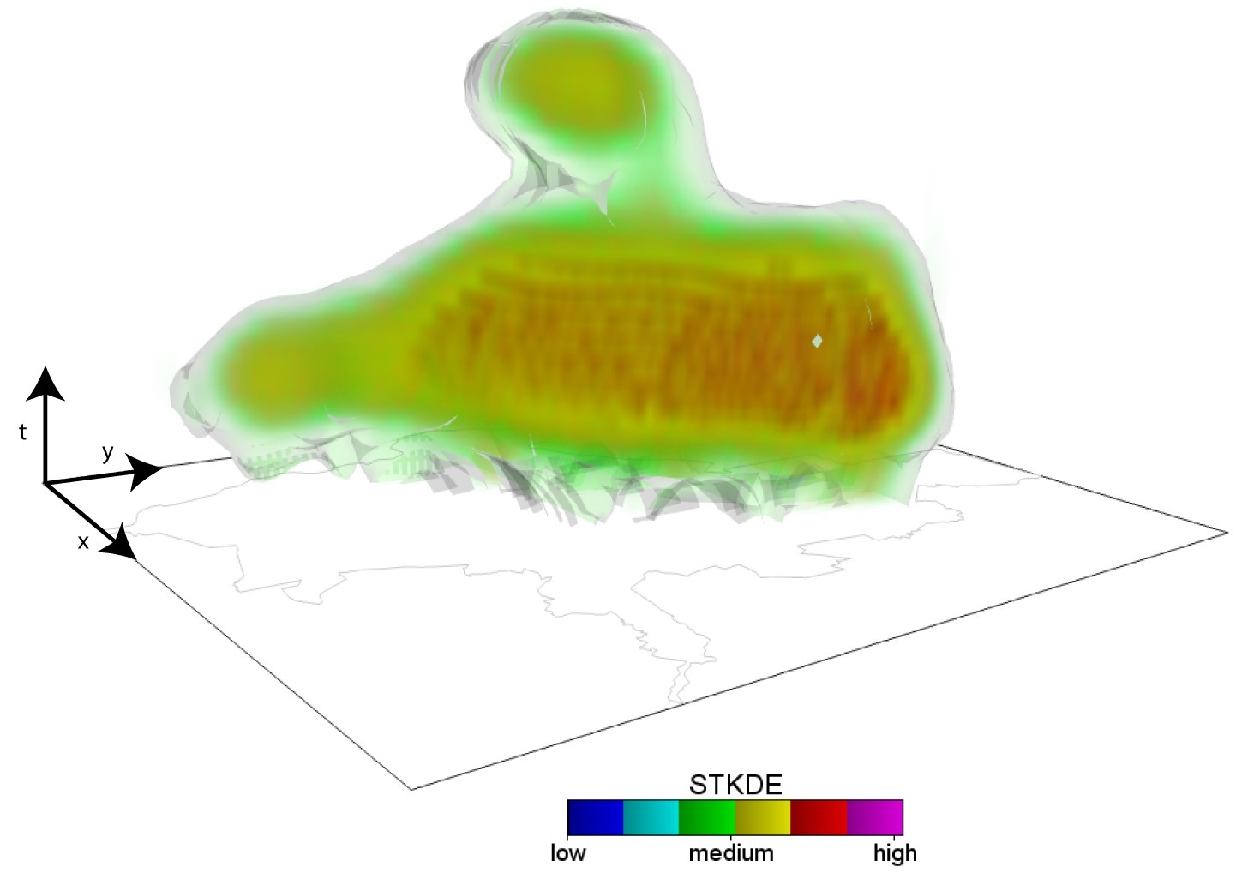
\includegraphics[width=.49\linewidth]{figures/Dengue-2500-14.pdf}}
%
%  \subfigure[$h_s=750m$, $h_t = 7 days$]{\includegraphics[page=2, width=.45\linewidth, trim={8cm 3.8cm 8cm 10cm}, clip]{figures/dengue-viz.pdf}}
\subfigure[$h_s=500m$, $h_t = 7 days$]{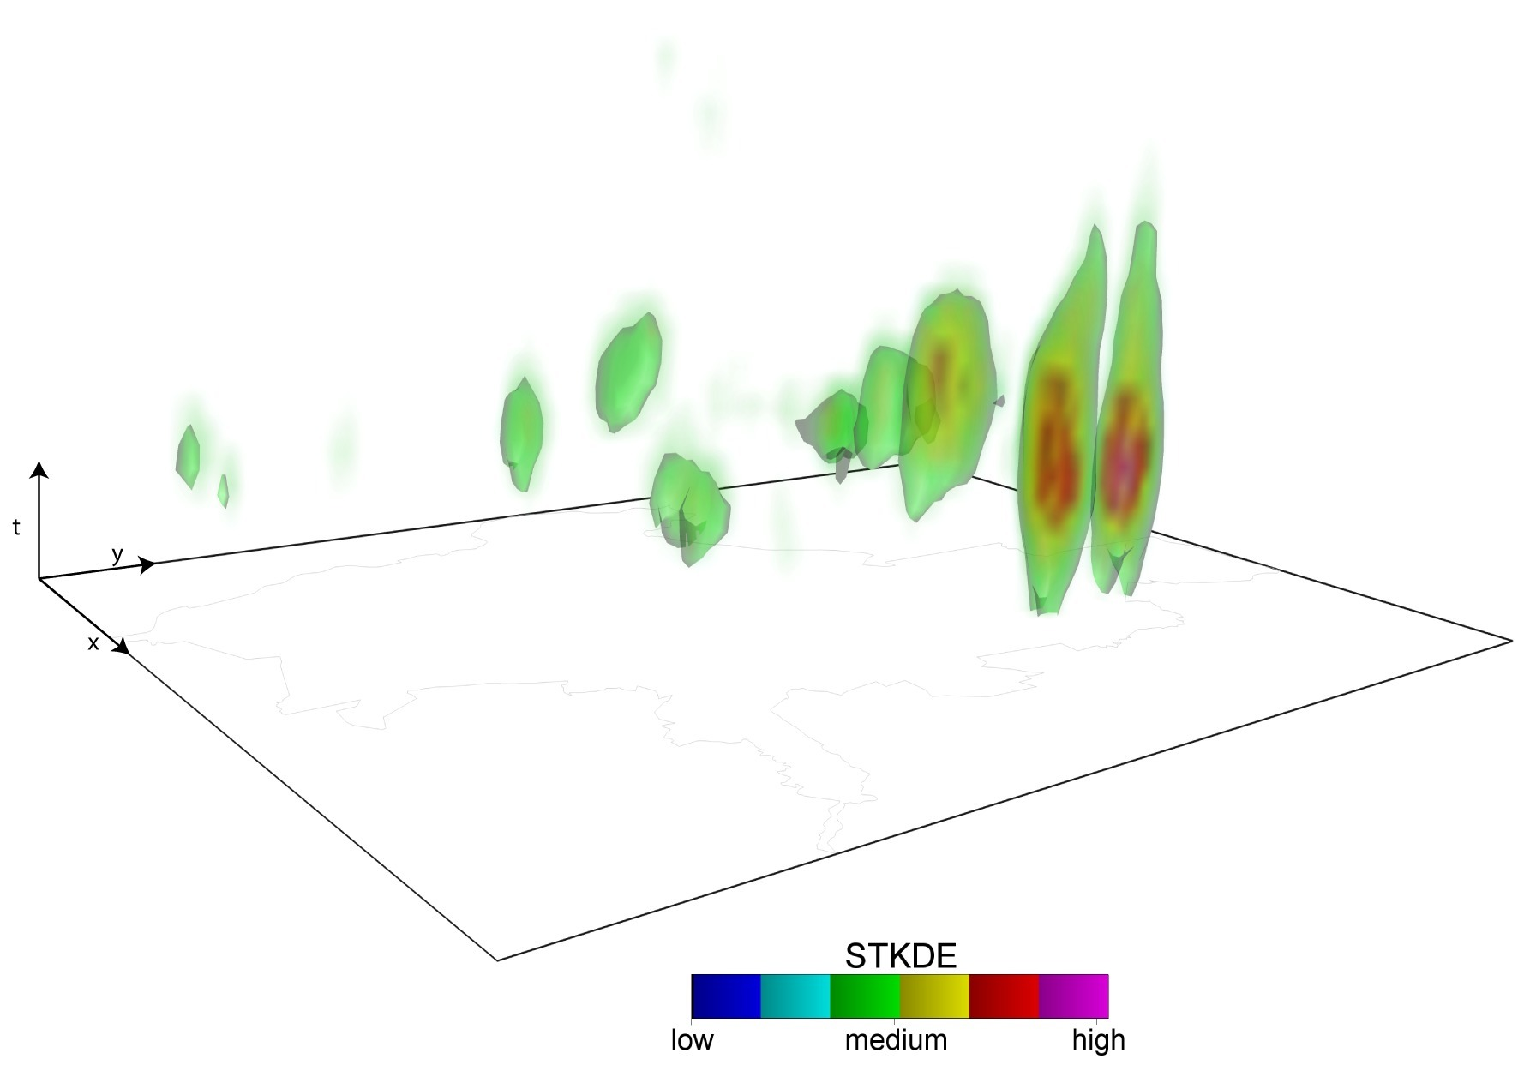
\includegraphics[width=.49\linewidth]{figures/Dengue-500-7.pdf}}
  \caption{Visualization of Dengue fever cases in Cali, Colombia in
    2010 and 2011 for different spatial bandwidth and temporal bandwidth.}
  \label{fig:stkde-ex}
\end{figure}

\begin{figure}
  \centering
  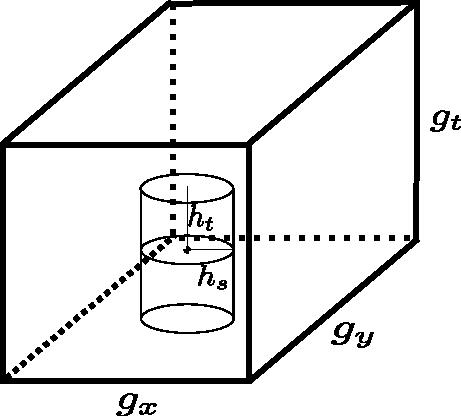
\includegraphics[width=.4\linewidth]{figures/stkde.pdf}
  \caption{The computation of STKDE happens in a domain space of size
    $g_x,g_y,g_t$. Each point impacts the neighboring space at a
    distance $h_s$ in space and $h_t$ in time; forming a cylinder of
    diameter $2 h_s$ and of height $2 h_t$.}
  \label{fig:stkde}
\end{figure}

Computationally, the domain of size $g_x$, $g_y$, $g_t$ is discretized
in voxels using a spatial resolution $sres$ and a temporal resolution
$tres$. Therefore, the domain is represented by a grid of size
$G_x=\ceil{\frac{g_x}{sres}}$, $G_y=\ceil{\frac{g_y}{sres}}$,
$G_t=\ceil{\frac{g_t}{tres}}$. Each point causes a density increase in
the voxels that are within a cylinder centered on the point, of
radius equal to the spatial bandwidth in voxels
$H_s=\ceil{\frac{h_s}{sres}}$, and of half height equal to the
temporal bandwidth $H_t=\ceil{\frac{h_t}{tres}}$.

All the notations are summarized in Table~\ref{tab:notation}. As a
convention all uppercase notations denote quantities in voxels and all
lowercase notations denote quantities in domain space.

\begin{table}
  \centering
  \begin{tabular}{|l|l|}
    \hline 
    $n$ & Number of points\\
    $s = (x,y,t)$ & A voxel and sampling coordinate\\
    $(x_i, y_i, t_i)$ & Coordinate of point $i$\\
    $h_s$, $h_t$ & Spatial and temporal bandwidth \\ 
    $g_x, g_y, g_t$ & Real size of the domain (in meters) \\
    \hline
    $sres$, $tres$ & Resolution (in meters) \\
    $s = (X,Y,T)$ & A voxel in voxel space\\
    $(X_i, Y_i, T_i)$ & Voxel of point $i$\\
    $G_x, G_y, G_t$ & Size of the domain (in voxels)\\
    $H_s, H_t$ & Bandwidth (in voxels) \\
    \hline 
  \end{tabular}
  \caption{Notations}
  \label{tab:notation}
  \vspace*{-3em}
\end{table}


\subsection{Point-based Algorithm}
The voxel-based algorithm suffers from a massive cost of computing
distances. The gold implementation reduces the number of distance computation by 
decomposing the domain, but that still incurs many distance calculations.
Most of these calculations are unnecessary since we know
where each point will radiate density. The point-based
algorithm PB, given in Algorithm~\ref{alg:pb}, leverages that
property.

\begin{algorithm}
\caption{\textsc{PB}}
\scriptsize
\begin{algorithmic}
\For{all voxels $s=(x,y,t)$}
  \State $stkde[X][Y][T] = 0$
\EndFor
%
\For{each points $i$ at $x_i, y_i, t_i$}
  \For{$X_i - H_s\leq X \leq X_i+H_s$}
    \For{$Y_i - H_s\leq Y \leq Y_i+H_s$}
      \For{$T_i - T_s\leq T \leq T_i+H_s$}
        \If{$\sqrt{(x_i-x)^2+(y_i-y)^2}< h_s$ and $|t_i-t| \leq h_t$}
        \State $stkde[X][Y][T] += \frac{k_s(\frac{x-x_i}{h_s},\frac{y-y_i}{h_s}) k_t(\frac{t-t_i}{h_t})}{n h_s^2h_t}$
        \EndIf
      \EndFor
    \EndFor
  \EndFor
\EndFor
\end{algorithmic}
\label{alg:pb}
\end{algorithm}

\todo{cut pba nd introduce directly PB-SYM}

The algorithm PB incurs mostly two costs. Initializing the memory which costs
$\Theta(G_x G_y G_t)$ and computing the impact of each point
$\Theta(n H_s^2 H_t)$. Note that it is possible that either of these
two terms is significantly larger than the other. Therefore the
complexity of the algorithm is $\Theta(G_x G_y G_t + n H_s^2 H_t)$.

\subsection{Exploiting Symmetries}

When the bandwidth is large, computing the density contribution of each
point each for voxel in the bandwidth is the most expensive
operation. Each of these $n (2  H_s)^2  2 H_t$ calculations costs
approximately 40 floating point operations. (The exact cost is
difficult to estimate since there are floating point additions,
multiplications, divisions, and square root operations).

One can remark that the calculation is mostly redundant since for one
particular point, its contribution to the neighboring voxels can be
decomposed in two components. $K_s(x,y)$  only depends on the
spatial coordinate of the voxel with respect to the point and does not
depend on its temporal coordinate. And $K_t(t)$  only depends on
the temporal coordinate and not on the spatial coordinates. See
Figure~\ref{fig:pb-sym-decomposition} for a graphical depiction.

\begin{figure}
  \centering
  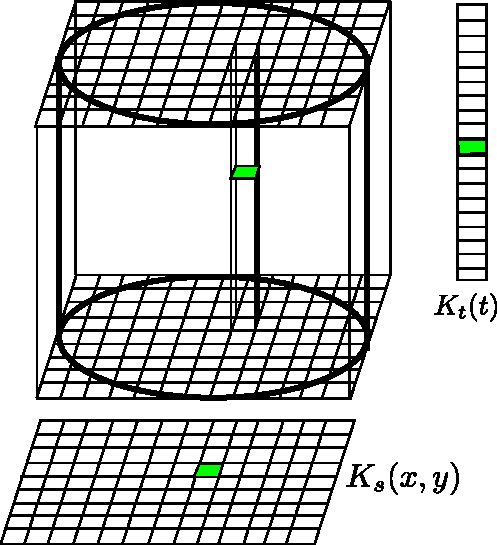
\includegraphics[width=.4\linewidth]{figures/PB-SYM.pdf}
  \caption{The contribution to the density estimate of each voxel of a
    cylinder can be decomposed in two terms, one temporally invariant
    $K_s(x,y)$ and one spatially invariant $K_t(t)$.}
  \label{fig:pb-sym-decomposition}
\end{figure}

Therefore, we write an algorithm to leverage these symmetries in
the problem. We present three variants, the PB-DISK variant ensures that
the invariant on the spatial domain is only computed once. The PB-BAR
variant ensures that the invariant on the temporal domain is only
computed once. The PB-SYM variant computes independently the spatial
invariant and the temporal invariant and then adds the density caused
by the point by taking the product of the two invariants. (See pseudocode in Algorithm~\ref{alg:pb-sym}.) 
Notice that leveraging the symmetries in the calculation does not change the
complexity (PB-SYM still has a complexity of $\Theta(G_x 
G_y  G_t + n  H_s^2  H_t)$) but reduces the number of flops.

\todo{cut discussion of PB-DISK and PB-SYM}

\begin{algorithm}
\caption{\textsc{PB-SYM}}
\scriptsize
\begin{algorithmic}
\For{all voxels $s=(x,y,t)$}
  \State $stkde[X][Y][T] = 0$
\EndFor
%
\For{each points $i$ at $x_i, y_i, t_i$}
  \For{$X_i - H_s\leq X \leq X_i+H_s$}
    \For{$Y_i - H_s\leq Y \leq Y_i+H_s$}
      \If{$\sqrt{(x_i-x)^2+(y_i-y)^2}< h_s$ }
        \State $K_s[X][Y] = \frac{k_s(\frac{x-x_i}{h_s},\frac{y-y_i}{h_s})}{n h_s^2h_t}$
      \Else
        \State $K_s[X][Y] = 0$
      \EndIf
    \EndFor
  \EndFor
  \For{$T_i - T_s\leq T \leq T_i+H_s$}
    \If{$|t_i-t| \leq h_t$}
      \State $K_t[T] = k_t(\frac{t-t_i}{h_t})$
    \Else
      \State $K_t[T] = 0$
    \EndIf
  \EndFor
%
  \For{$X_i - H_s\leq X \leq X_i+H_s$}
    \For{$Y_i - H_s\leq Y \leq Y_i+H_s$}
      \For{$T_i - T_s\leq T \leq T_i+H_s$}
        \State $stkde[X][Y][T] +=  K_s[X][Y] K_t[T]$
      \EndFor
    \EndFor
  \EndFor
\EndFor
\end{algorithmic}
\label{alg:pb-sym}
\end{algorithm}

\label{sec:algo-pb-sym}

\todo{shorten and rephrase for IPDPS}

\todo{Point to ICPP paper for detail of performance difference}

\subsection{Domain Decomposition}

 strategy to avoid the data race is to compute 
voxel intensity  independently for different subdomains. We call this method PB-SYM-DD (Algorithm~\ref{alg:pb-sym-dd}).
It splits the domain in AxBxC subdomains and each subdomain is
associated the points which cylinder intersects with a voxel of
the subdomain. Then the algorithm proceeds with handling each
subdomain independently by only considering the impact of the
data-point on voxels within the subdomain.

\begin{algorithm}
\caption{\textsc{PB-SYM-DD}}
\scriptsize
\begin{algorithmic}
\For{all points $i=(x_i,y_i,t_i)$}
  \For{each subdomain $(a,b,c)$}
        \If{$(X,Y,T) \pm (H_s,H_s,H_T)$ intersects \\$(\floor{\frac{a G_x}{A}}:\ceil{\frac{(a+1) G_x}{A}}, \floor{\frac{b G_y}{B}}:\ceil{\frac{(b+1) G_y}{B}}, \floor{\frac{c G_t}{C}}:\ceil{\frac{(c+1) G_t}{C}})$}
          \State $localpoints[a][b][c].add(x_i,y_i,t_i)$
        \EndIf
  \EndFor
\EndFor
%
\For{each subdomain $(a,b,c)$ in parallel}
  \State Process subdomain $(a,b,c)$ using PB-SYM
\EndFor
\end{algorithmic}
\label{alg:pb-sym-dd}
\end{algorithm}

The main problem with Domain Decomposition is that it requires some
points to be replicated across multiple subdomain which incurs
additional work. Indeed, if a point is replicated in multiple subdomains,
its cylinder is split across multiple subdomains as well. Assuming the split is
temporal, then using PB-SYM in each subdomain requires computing
part of the temporal invariant, the entire spatial invariant, and part
of the cylinder. Therefore both subdomains need to compute the entire
spatial invariant. See Figure~\ref{fig:pb-sym-dd-overhead} for a
graphical depiction of this phenomenon.

\begin{figure}
  \centering
  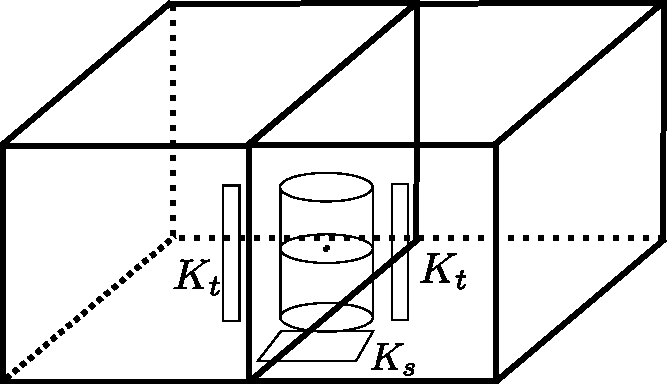
\includegraphics[width=.5\linewidth]{figures/PB-SYM-DD-overhead.pdf}
  \caption{When a cylinder is split among two subdomains, PB-SYM-DD
    causes an overhead because one of the invariant needs to be
    recomputed. Here each subdomains compute part of the temporal
    invariant $K_s$, but both need to compute the spatial invariant $K_t$.}
  \label{fig:pb-sym-dd-overhead}
\end{figure}

If the algorithms keeps the number of subdomains small such that each
point is replicated less than a constant number of times, then
the work expressed in Big-Oh notation does not change.
(This can be achieved by having subdomains larger than
$H_s \times H_s \times H_t$.) However, the practical amount of work can
increase by a non-negligable factor. 

Another issue with Domain Decomposition is load imbalance. The
points are unlikely to be equally distributed in the domain space, but
more likely clustered around some locations. The subdomain containing
a cluster will have a significantly higher work than other
subdomains. And this work is not executed in parallel. One could
decompose the domain more, but replicated point 
will incur an even higher overhead which may end up nullifying
the gain in load balance.\looseness=-1

\todo{intoduce model}

\section{Exact Decomposition}
\label{sec:exactdecomposition}




\section{Overdecomposition}
\label{sec:overdecomposition}


\section{Experiments}
\label{sec:experiments}

\section{Conclusion}
\label{sec:ccl}

\section*{Acknowledgment}
Thanks to Bora Ucar for some discussion on this problem. This material
is based upon work supported by the National Science Foundation under
Grant No. 1652442.

\bibliographystyle{IEEEtran}
\bibliography{ipdps}


\end{document}
